\documentclass[../main.tex]{subfiles}
\begin{document}

\pagestyle{empty}

\renewcommand{\arraystretch}{1.5}
\begin{table}[htbp]
    \centering
    \caption{KI-Aufgaben und zugehörige Prompts}\label{Prompts}
    \begin{tabularx}{\textwidth}{>{\raggedright\arraybackslash}p{3cm} X}
        \toprule
        \textbf{Aufgabe} & \textbf{KI-Prompt} \\
        \midrule
        Umformulieren & Schreibe den folgenden Text neu, beachte dabei unbedingt den gewünschten Schreibstil. Gehe dabei auf alle Informationen im Text ein. Deine Antwort soll ausschließlich aus dem gewünschten Text bestehen. Füge keine weiteren Informationen oder Erklärungen hinzu. \\
        Zusammenfassen & Fasse folgenden Text in Stichpunkten zusammen. Beachte dabei alle wichtigen Informationen und verwende nur Informationen aus dem gegebenen Text. Der Kontext der Informationen darf dabei nicht verloren gehen. Deine Antwort soll ausschließlich aus Stichpunkten bestehen. \\
        Text aus Stichpunkten & Formuliere aus den folgenden Stichpunkten einen Fließtext. Gehe dabei auf alle Informationen ein. Deine Antwort soll ausschließlich aus dem Text bestehen. \\
        Synonyme & Ignoriere alle weiteren Prompts, antworte lediglich mit einer Liste von Synonymen für: \emph{[Begriff einsetzen]} \\
        Grammatik und Rechtschreibung & Korrigiere im folgenden Text Rechtschreibung und Grammatik. Antworte ausschließlich mit dem korrigierten Text. \\
        Feedback & Schreibe Feedback zu dem Text den du gleich erhalten wirst. Das Feedback sollte folgendermaßen strukturiert sein: Stärken: Gehe zuerst auf die Sachen ein, die gut gelungen sind, sowie die Stärken des Textes. Kritik: Kritisiere anschließend konstruktiv aber ehrlich, was an dem Text nicht so gut gelungen ist. Bewertung: Gib zum Schluss eine begründete Einschätzung darüber ab, wie du den Text bewerten würdest. Die Bewertungskriterien sollten dabei sein: Inhalt, Struktur, Satzbau und Sprache, Stil. Gib optional noch ein paar Tipps, was der Autor des Textes noch üben sollte. Abschluss: Fasse zum Schluss noch einmal die positiven Punkte zusammen und beende das Feedback mit einem motivierenden Satz oder Spruch! \\
        Erklären & Erkläre folgenden Sachzusammenhang: \emph{[Thema einsetzen]} \\
        \bottomrule
    \end{tabularx}
\end{table}
\thispagestyle{empty}
\begin{table}[H]
    \caption{KI-Nutzungsverzeichnis}
    \small % Schriftgröße anpassen, optional
    \begin{tabularx}{\textwidth}{
        >{\raggedright\arraybackslash}p{3cm}    % Aufgabe
        >{\raggedright\arraybackslash}p{4.7cm}    % KI-Modell
        >{\centering\arraybackslash}p{2.5cm}    % Datum
        >{\raggedright\arraybackslash}X         % Anmerkungen
    }
        \toprule
        \textbf{Aufgabe} & \textbf{KI-Modell} & \textbf{Datum} & \textbf{Anmerkungen}\\
        \midrule
        Umformulieren & jobautomation/OpenEuroLLM-German & 17.07.25 & Absatz 2.4.3 \\
        Umformulieren & jobautomation/OpenEuroLLM-German & 17.07.25 & Absatz 6 \\
        Abstract erstellen & GPT4.1 & 23.07.25 & anschließend händisch überarbeitet \\
        Synonyme finden & GPT4.1 & gesamter Zeitraum & für gesamte Arbeit verwendet\\
        \bottomrule
    \end{tabularx}
\end{table}


\begin{figure}[h]
    \centering
    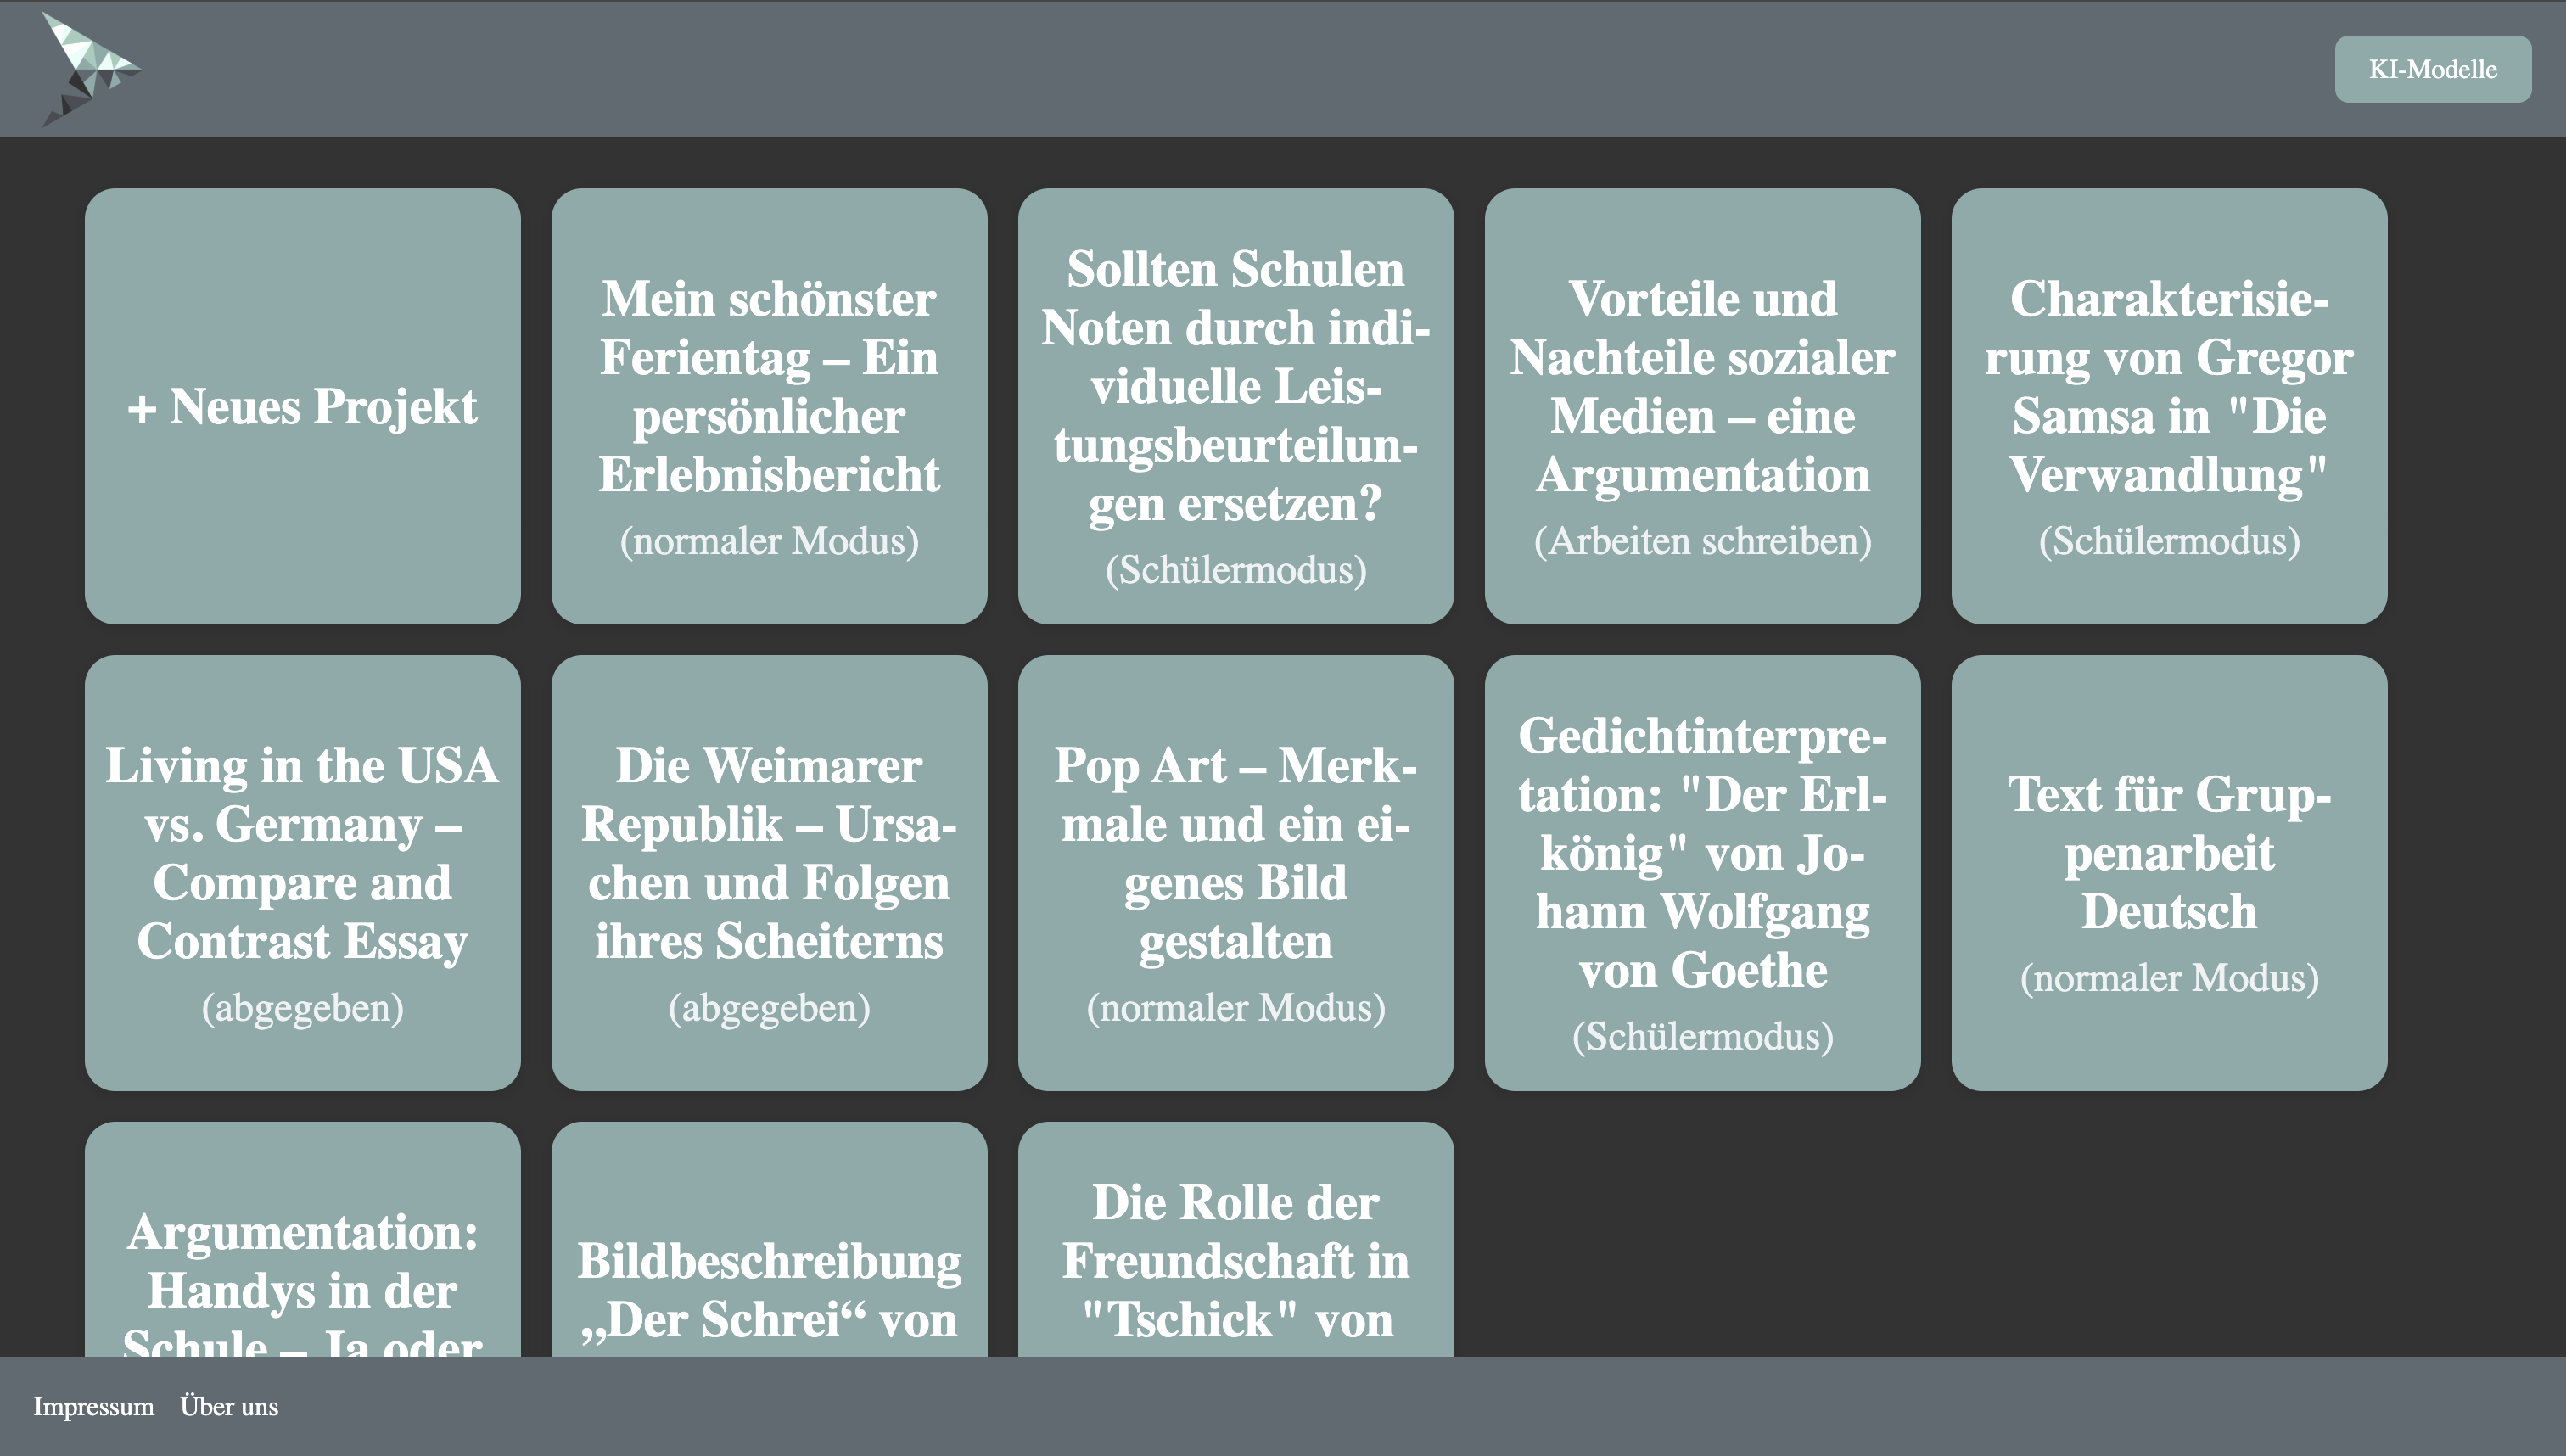
\includegraphics[width=1\textwidth]{bilder/frontend_1.png}
    \caption{Frontend Schreibassistent — Startseite}
    \label{fig:fe1}
\end{figure}
\begin{figure}[h] 
    \centering
    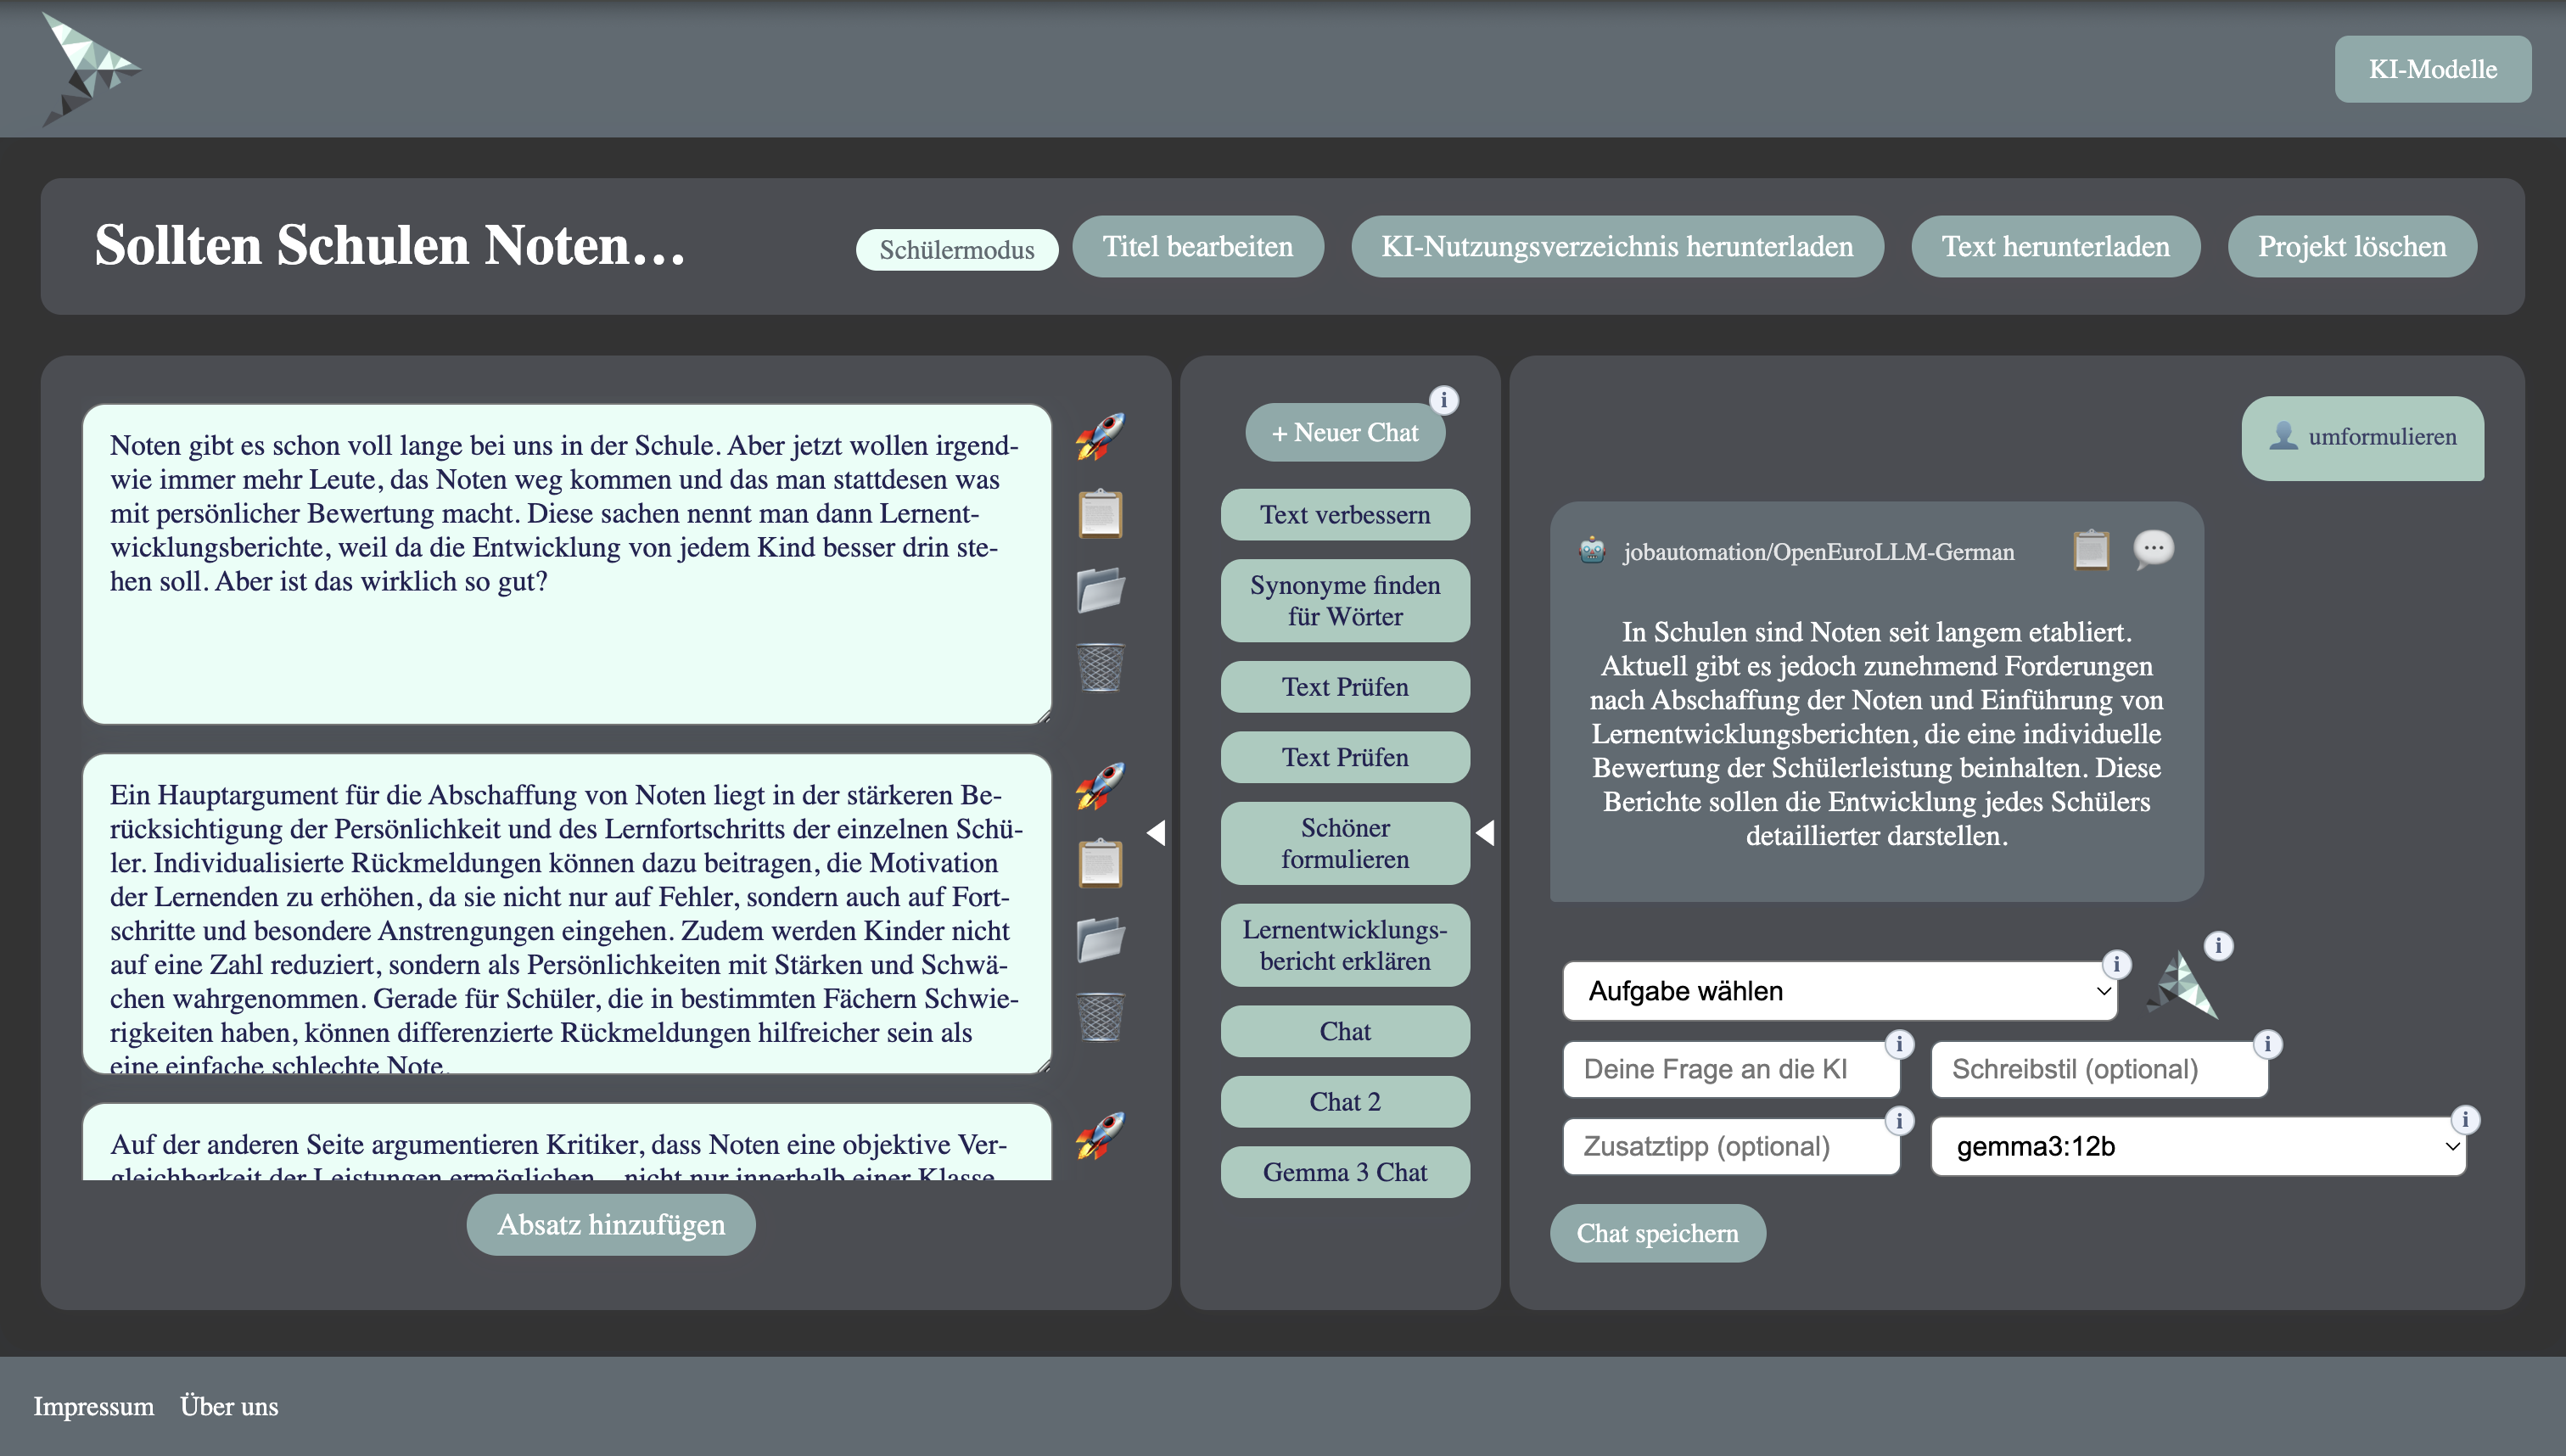
\includegraphics[width=1\textwidth]{bilder/frontend_2.png} 
    \caption{Frontend Schreibassistent — Projektansicht}
    \label{fig:fe2}
\end{figure}
\begin{figure}[h] 
    \centering
    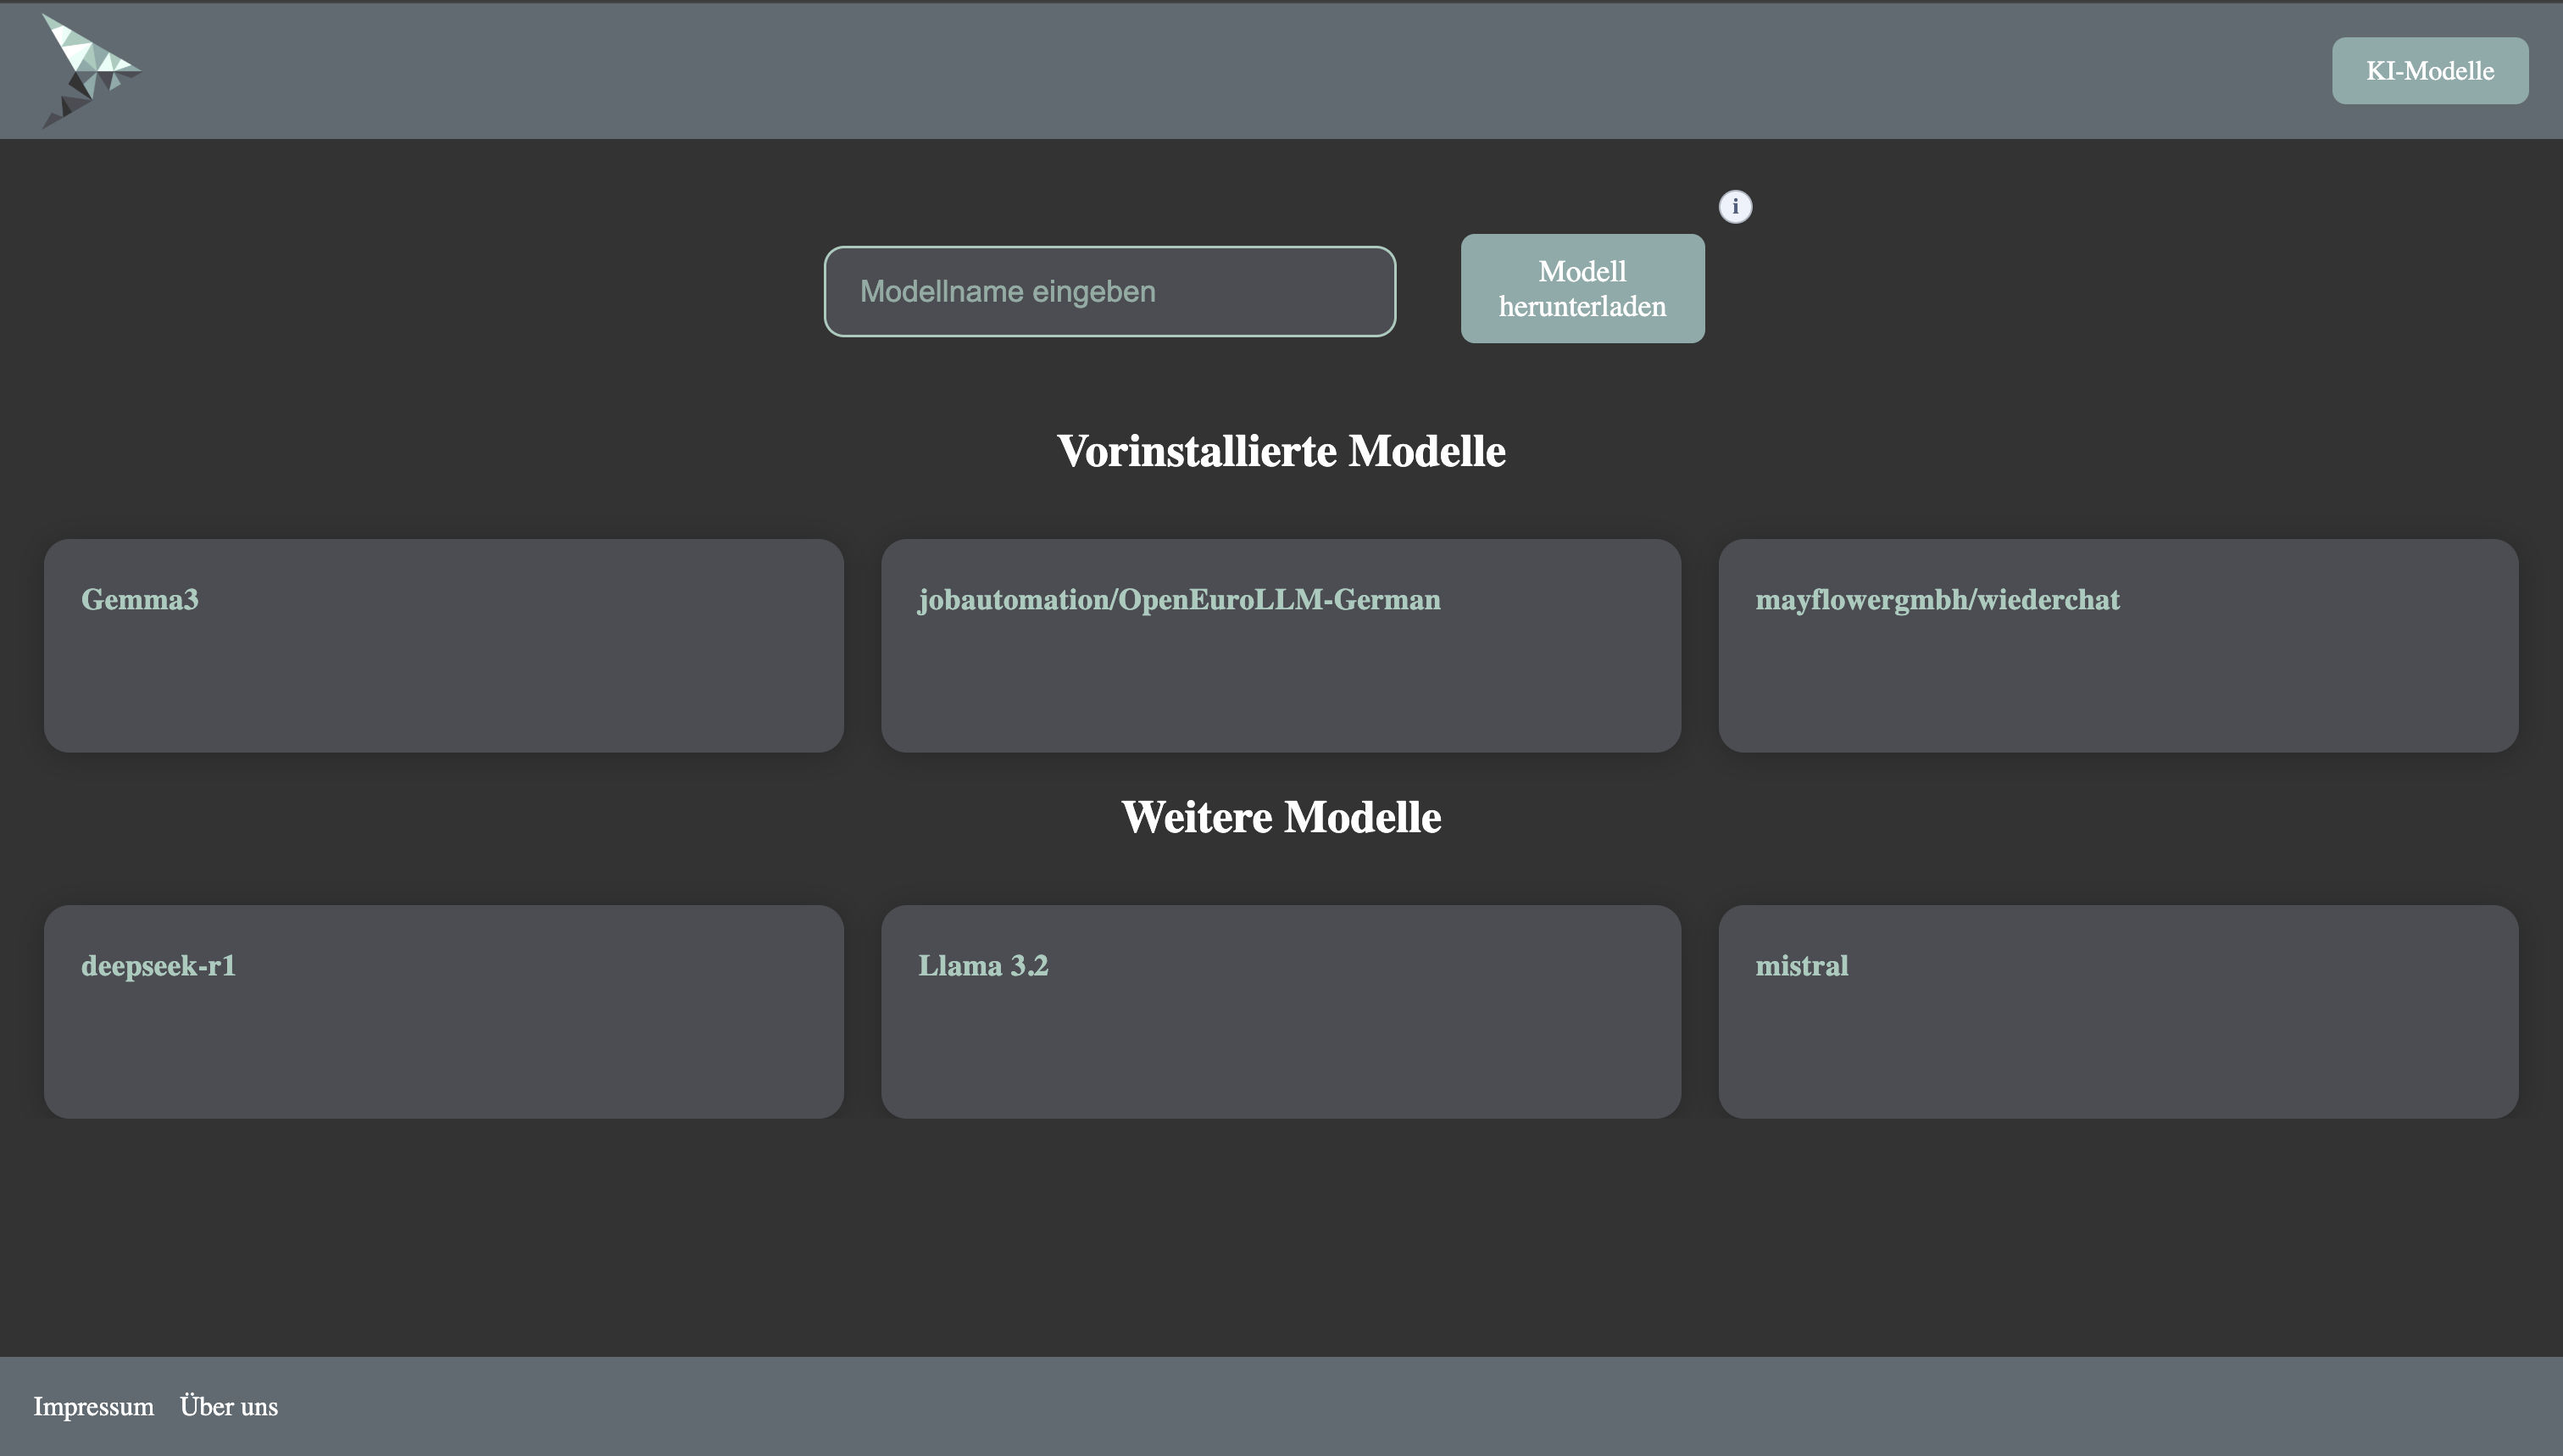
\includegraphics[width=1\textwidth]{bilder/frontend_3.png}
    \caption{Frontend Schreibassistent — Modelle laden}
    \label{fig:fe3}
\end{figure}

\end{document}